\documentclass[10pt,a4paper,twocolumn]{article}
\usepackage[utf8]{inputenc}
\usepackage{amsmath}
\usepackage{amsfonts}
\usepackage{amssymb}
\usepackage{graphicx}
%\usepackage{hyperref}
\usepackage{cleveref}
%\usepackage{multicol}

%\usepackage[backend=bibtex,style=numeric,sorting=none]{biblatex}
\usepackage[backend = bibtex,style=phys, articletitle=false,  biblabel=brackets, sorting=none]{biblatex}
\usepackage{authblk}

\DeclareFieldFormat{journaltitle}{\mkbibemph{#1}}
\DeclareFieldFormat{pages}{#1}
\DeclareFieldFormat{booktitle}{\mkbibemph{#1}}



%\bibliographystyle{numeric}
\bibliography{chgcnn}

\makeatletter
\renewcommand{\@seccntformat}[1]{}
\makeatother

\usepackage{fullpage}


\title{Crystal Hypergraph Convolutional Networks}
\author{
Alexander J. Heilman, Weiyi Gong, and Qimin Yan
  }
  
\date{}

\affil{\textit{
Department of Physics}\\
\textit{Northeastern University, 
Boston, MA 02115, USA}}

\begin{document}
\twocolumn[
\maketitle
  \begin{@twocolumnfalse}
    \maketitle
    \begin{abstract}
    ADD corresponding author...
    	
    Graph representations of solid state materials that encode only interatomic-distance information lack geometrical resolution, resulting in degenerate representations that may map distinct structures to equivalent graphs. Here we propose a hypergraph representation scheme for materials that allows for the association of higher-order geometrical information with hyperedges. Hyperedges generalize edges to connected sets of more than two nodes, and may be used to represent triplets and local environments of atoms in materials. This generalization of edges requires a different approach in graph convolution, three of which are developed in this work. These crystal hypergraph convolutional networks are trained based on various property prediction tasks for a vast set of solid-state materials in the Materials Project and MatBench databases. Results presented here focus on the improved performance of models based on both pair-wise edges and local environment hyperedges. These results demonstrate that hypergraphs are an effective and efficient method for incorporating geometrical information in material representations.
    \end{abstract}
  \end{@twocolumnfalse}
  \vspace{.5cm}
]


\section{Introduction}
Machine learning has proven to be a computationally cost-effective and powerful predictive tool in the screening of large sets of material systems for certain material properties \cite{mlcite1, mlreview1, mlreview2, mlreview3}. Some of the most effective state-of-the-art models applied to invariant target predictions represent material systems as graphs \cite{schnet, cgcnn, megnet, chemgnn, geocgcnn, icgcnn}. These graphs encode physical properties in feature vectors associated with graph components, and update or `learn' these features with a trained graph neural network or message passing network \cite{mpnn}. 

One problem with such graphical representations, however, is the lack of representation of higher-order geometrical structure, since the constructed crystal graphs can only include pair-wise descriptors. This may make it difficult or even impossible for models to distinguish between compositionally similar but structurally distinct systems with unique material properties \cite{congn}. Other works have approached this problem by including higher-order geometrical features such as overlapping bonds' angles \cite{alignn,m3gnet,congn}. However, these approaches come with an increase in the total number of messages exchanged through convolution that is quadratic with respect to $\Bar{N}_{\text{edges}}$, the average number of edges per atom.

Here, we propose the concept of \textit{crystal hypergraphs} to address this lack of geometrical information in the more restrictive graph representations. In a crystal hypergraph, we may define larger (than strictly pair-wise) hyperedges that correspond to higher-order geometrical structures of material systems explicitly, such as triplets of neighboring atoms, or coordination polyhedra/motifs \cite{paulings_rules, coordpolyshapes, motifstats, motifexplore, clustermotifsanal, motife3nn}. These different structures then may have different coordinate invariant features associated with them, such as angles and local order parameters \cite{orderparam1, orderparam2, molorderparam}, respectively. Note that in that regard, crystal hypergraphs are naturally heterogeneous in their hyperedges, since there are different feature sets for different types of hyperedges.

Of course, the definition of a more general hypergraph representation requires the generalization of the message passing framework mentioned above. Here, we propose three possible approaches to such a generalization that handle the now-variable size of hyperedges. In a certain sense, these allow for the learning of a certain type of `cluster-correlation expansion' (CCE) \cite{clease, cce_crys, cce_gen, wu2016cluster} by the model, where clusters of interest correspond to the hyperedges defined. Indeed, atomic cluster expansions have previously been utilized, to great effect, in the generation and application of transferable interatomic potentials \cite{ace, ace_completeness, ace_appplication} and are also motivated by lattice-based cluster expansion methods.

In many-body expansions, such as CCE, expansions are often truncated to exclude higher-order terms since their associated parameters are typically observed to decay quickly with increasing distance from the central atom. Similarly, in multi-pole expansions, higher-order terms (such as quadrupole, octupole, and beyond) often contribute considerably less to long-range field effects. The intuition gained from these considerations further support the use of only a localized set of descriptors for atom-centric models. This intuition is used in the present work to motivate the use of neighborhood aggregation for hyperedge message passing, wherein only atomic features local to hyperedges are incorporated in their associated messages.

As a proof of concept, we propose and implement a crystal hypergraph convolutional model (CHGCNN) that incorporates invariant geometric features for bonds, triplets, and motifs in crystals as hyperedge features. This provides us a unique opportunity to demonstrate the importance of different order structures for these different material property prediction tasks. Namely, we compare the performance of models based on atom, bond, and triplet information against those incorporating atom, bond, and motif information (i.e. first shell hyperedges) on various predictive tasks with varying data sizes.

Results presented here indicate that first-shell (motif) hyperedges may be sufficient, if not more informative, than triplet hyperedges for many common predictive tasks. This comes at a substantially lower computational cost, in terms of the total number of messages exchanged through graph convolution.

The structure of this work is as follows. We give a brief overview of crystal graph construction and message passing networks. A motivating representation problem is then identified with our definitions and the concept of crystal hypergraphs is introduced, with a particular focus on different types of hyperedges and their corresponding feature sets. Three generalized message passing frameworks are then considered, and a specific model architecture is presented. Finally, this specific architecture is used on various datasets to evaluate the performance of different sets of hyperedge types.

Other works consider a similar problem in spirit, namely, how to more effectively and efficiently describe the geometric features of material systems beyond simple pair-wise features as in graph neural networks. In particular, molecular graph coarsening models \cite{molgraphcoarse1} aim to be more efficient in their descriptors, and hence representations, by coarsening the graphs representing molecular systems through convolution, aiming to keep only the most important groupings. Another common approach is to directly incorporate the directional vectors of edge features and maintain equivariance through convolution \cite{nequip, tfn, e3nn}, though this requires substantially different convolutional architectures than those adopted in invariant networks, often at a higher computational cost though with the additional ability to directly predict coordinate-system dependent quantities.

\section{Background}
\subsection{Crystal Graphs}
A common representation of crystalline systems in machine learning is via graphs (that is, collections of nodes and binary connections between them). We may define a crystal graph $\mathcal{G}=\lbrace \mathcal{V},\mathcal{E}\rbrace$ as a set of vertices $v_i\in\mathcal{V}$, corresponding to each atom $i$, and edges $e_{ij}\in\mathcal{E}$, where edges are determined by some physical criteria. Physical information is then associated with the objects in these graphs by way of feature vectors. These are vectors with components describing the physical characteristics of their corresponding graph component, and which may be further 'learned' or updated through a graph neural network.

%Below, we give a typical approach for the construction of crystal graphs. Note, however, that while this section is meant to exemplify other works' approaches, we also use the following in the first step of crystal hypergraph generation.

%\subsection{Crystal Graph Edge Criteria}
A commonly applied criterion for the formation of edges between atoms is a combination of a maximum distance cutoff $r_{max}$ and a maximum number of neighbors for each node $N_{max}$. That is, for each atom, edges are constructed between its node and its $\leq N_{max}$-th closest neighbors in the crystalline structure within a shell of radius $r_{max}$.

%While other criteria may also be utilized, such as face-sharing in Voronoii Tesselations, and scaled maximum distance cutoffs based on nearest neighbor distances, these more advanced criteria are generally more computationally expensive in the data processing stage and often provide negligible differences in performance. Alternatively, most models \cite{cgcnn,alignn,megnet} adopt the more basic criteria of maximum numbers of neighbors within cutoff shells, and adopt some continuous-filter convolutional function that can learn which connections are more important for the task at hand.

%Often, this maximum number of neighbors considered is chosen to be $12$, however recent tests in coNGN \cite{congn} suggest even this may be too restrictive, and show that a maximum set as large as 24 may improve performance.

%As a maximum distance cutoff, since we focus primarily on crystalline structures here, we consider $6$ \AA $ $  to be sufficient.

%\subsection{Crystal Graph Features}
The nodes' feature vectors encode the atomic information of the sites they describe. Two usual techniques include: explicitly engineered feature vectors (as in \cite{cgcnn}); and the learning of encodings for atomic sites based only on their atomic number (as in \cite{megnet}), beginning with some random initialization. Edge features are often derived exclusively from their distance.


%%%move to later construction
%Note that we could also, in principle, include an atomic position in the node features. However, this would require a special treatment of such information through convolution if we wished to maintain an \textit{invariant} representation up to choice of coordinate system. As such, often only coordinate system (or more specifically, Euclidean group) invariant features are included in crystal graph representations. This restriction to invariant features also precludes any inclusion of unit vector orientation in edge features which are discussed below.





%\subsection{Crystal Graph Convolution}
Crystal graphs are usually constructed solely for use in graph convolutional neural networks. Perhaps the most general framework in which we may define graph convolution is the message passing framework defined by Gilmore \cite{mpnn}.
A message passing network updates nodes based on 'messages' generated by the features of, and passed through, neighboring nodes (that is, nodes sharing an edge).% Gilmore defines the message passing framework in terms of three functions: $M$, the message forming function; $U$, the node update function; and $R$, the readout function. 


%Message passing networks acting on crystal graphs have several advantages: message passing networks enjoy invariance under permutation of node indices; and, further, if the encoded features are coordinate system invariant, the output of the network is itself coordinate system invariant.


%\subsection{Disadvantages of Crystal Graphs}

However, the construction above lacks higher-order geometrical information within the crystals. That is, distinct local geometrical environments of atoms (motifs) may be mapped degenerately to the same crystal graph.
As a simple example of the low resolution manifest in crystal graphs, consider two atomic systems below: one with a local cubic symmetry, and another with a square anti-prism local environment; but both with the same bonding atoms. As demonstrated in Figure \ref{fig:graph_cntex} both structures would map to the same crystal graph, but could be easily distinguished with an additional descriptor describing the local geometry of each central atom.

Alternatively, one could include atomic position in the node features or a vector direction in edge features. However, this generally requires a unique treatment of such coordinate-system dependent information through convolution if the output is to maintain \textit{invariance} with respect to changes in the coordinate system. As such, often only coordinate system invariant features are included in crystal graph representations, such as distance and atomic properties. 

\begin{figure*}
	\centering
	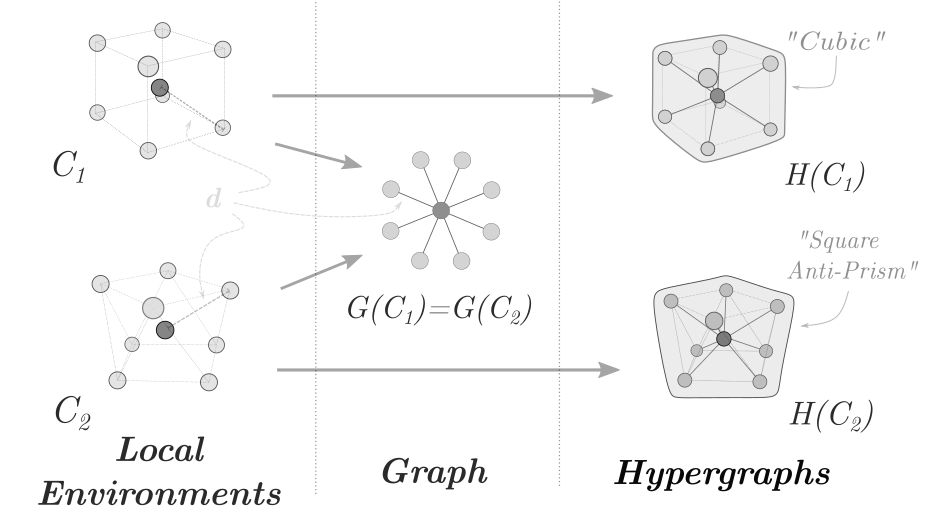
\includegraphics[scale=0.64]{graph2hgraph_tall_revise2.pdf}
	\caption{An example of two distinct geometries that are mapped to the same distance-based crystal graph. With inclusion of a first-shell feature vector encoding local geometry however, these structures are mapped to two distinct crystal hypergraphs. Note these are two possible coordination environments in oxides, determined statistically in \cite{motifstats}.}
	\label{fig:graph_cntex}
\end{figure*}

\section{Methods}

\subsection{Crystal Hypergraph Construction}
Hypergraphs are a very general framework describing relations between an abstract set $\mathcal{V}$ of nodes or vertices, defined by by a set of hyperedges $\mathcal{H}$ containing arbitrary subsets of $\mathcal{V}$. Consequently, the set of all hypergraphs on a set of nodes is more general than, and contains all possible, topological sets and simplicial complexes on $\mathcal{V}$ \cite{Mulas2022}. The method proposed here reduces the intrinsic limitations of invariant crystal graph features by allowing the explicit incorporation of higher-order geometrical information in the form of hyperedges, which can be used to directly represent these higher-order structures. Furthermore, the more general definition of hypergraphs allows for complete freedom in the choice of structures to be included, as opposed to the more rigid definition and utilization of representations in simplicial-complex networks \cite{equivariant_simplices, simplicial_networks}.

A crystal hypergraph $\mathcal{H}=\lbrace\mathcal{V}, \mathit{H} \rbrace$ is a collection of nodes $v_i\in \mathcal{V}$ and hyperedges $h_j\in \mathit{H}$ (containing an arbitrary number of nodes, see Supplementary Note S5), where the hyperedges are most generally heterogeneous. That is, we generally wish to describe different types of hyperedges (e.g. bonds, triplets, and motifs) in the same crystal hypergraph. These objects then have associated feature vectors encoding relevant physical information, which we also refer to as $v_i$ and $h_j$, since the indices specify all the relevant information for their association to particular nodes and hyperedges, respectively.

For the purpose of modeling material systems, we need to identify what different order structures are most important in their representation. Of course, atomic and bond level information is particularly important. However, higher-order structures may also be of interest, such as triplets of atoms and local environments of atoms, which we refer to as motifs in crystals.

Each of the aforementioned structures also has a natural set of distinct, coordinate-system invariant features that may be associated with them. At the triplet level (where two bonds share some common node), there is always a corresponding angle. While at the motif level, order parameters \cite{orderparam1, orderparam2} or continuous symmetry measures \cite{csm_polyhedra, chemenv} may be used to describe 3-dimensional coordination environments quantitatively. 
These different order structures may all be represented in a single crystal hypergraph. 
Below, we discuss the generation of, and association of features with, all of the above-mentioned structures in crystalline solids. 

\begin{figure*}[!ht]
	\centering
	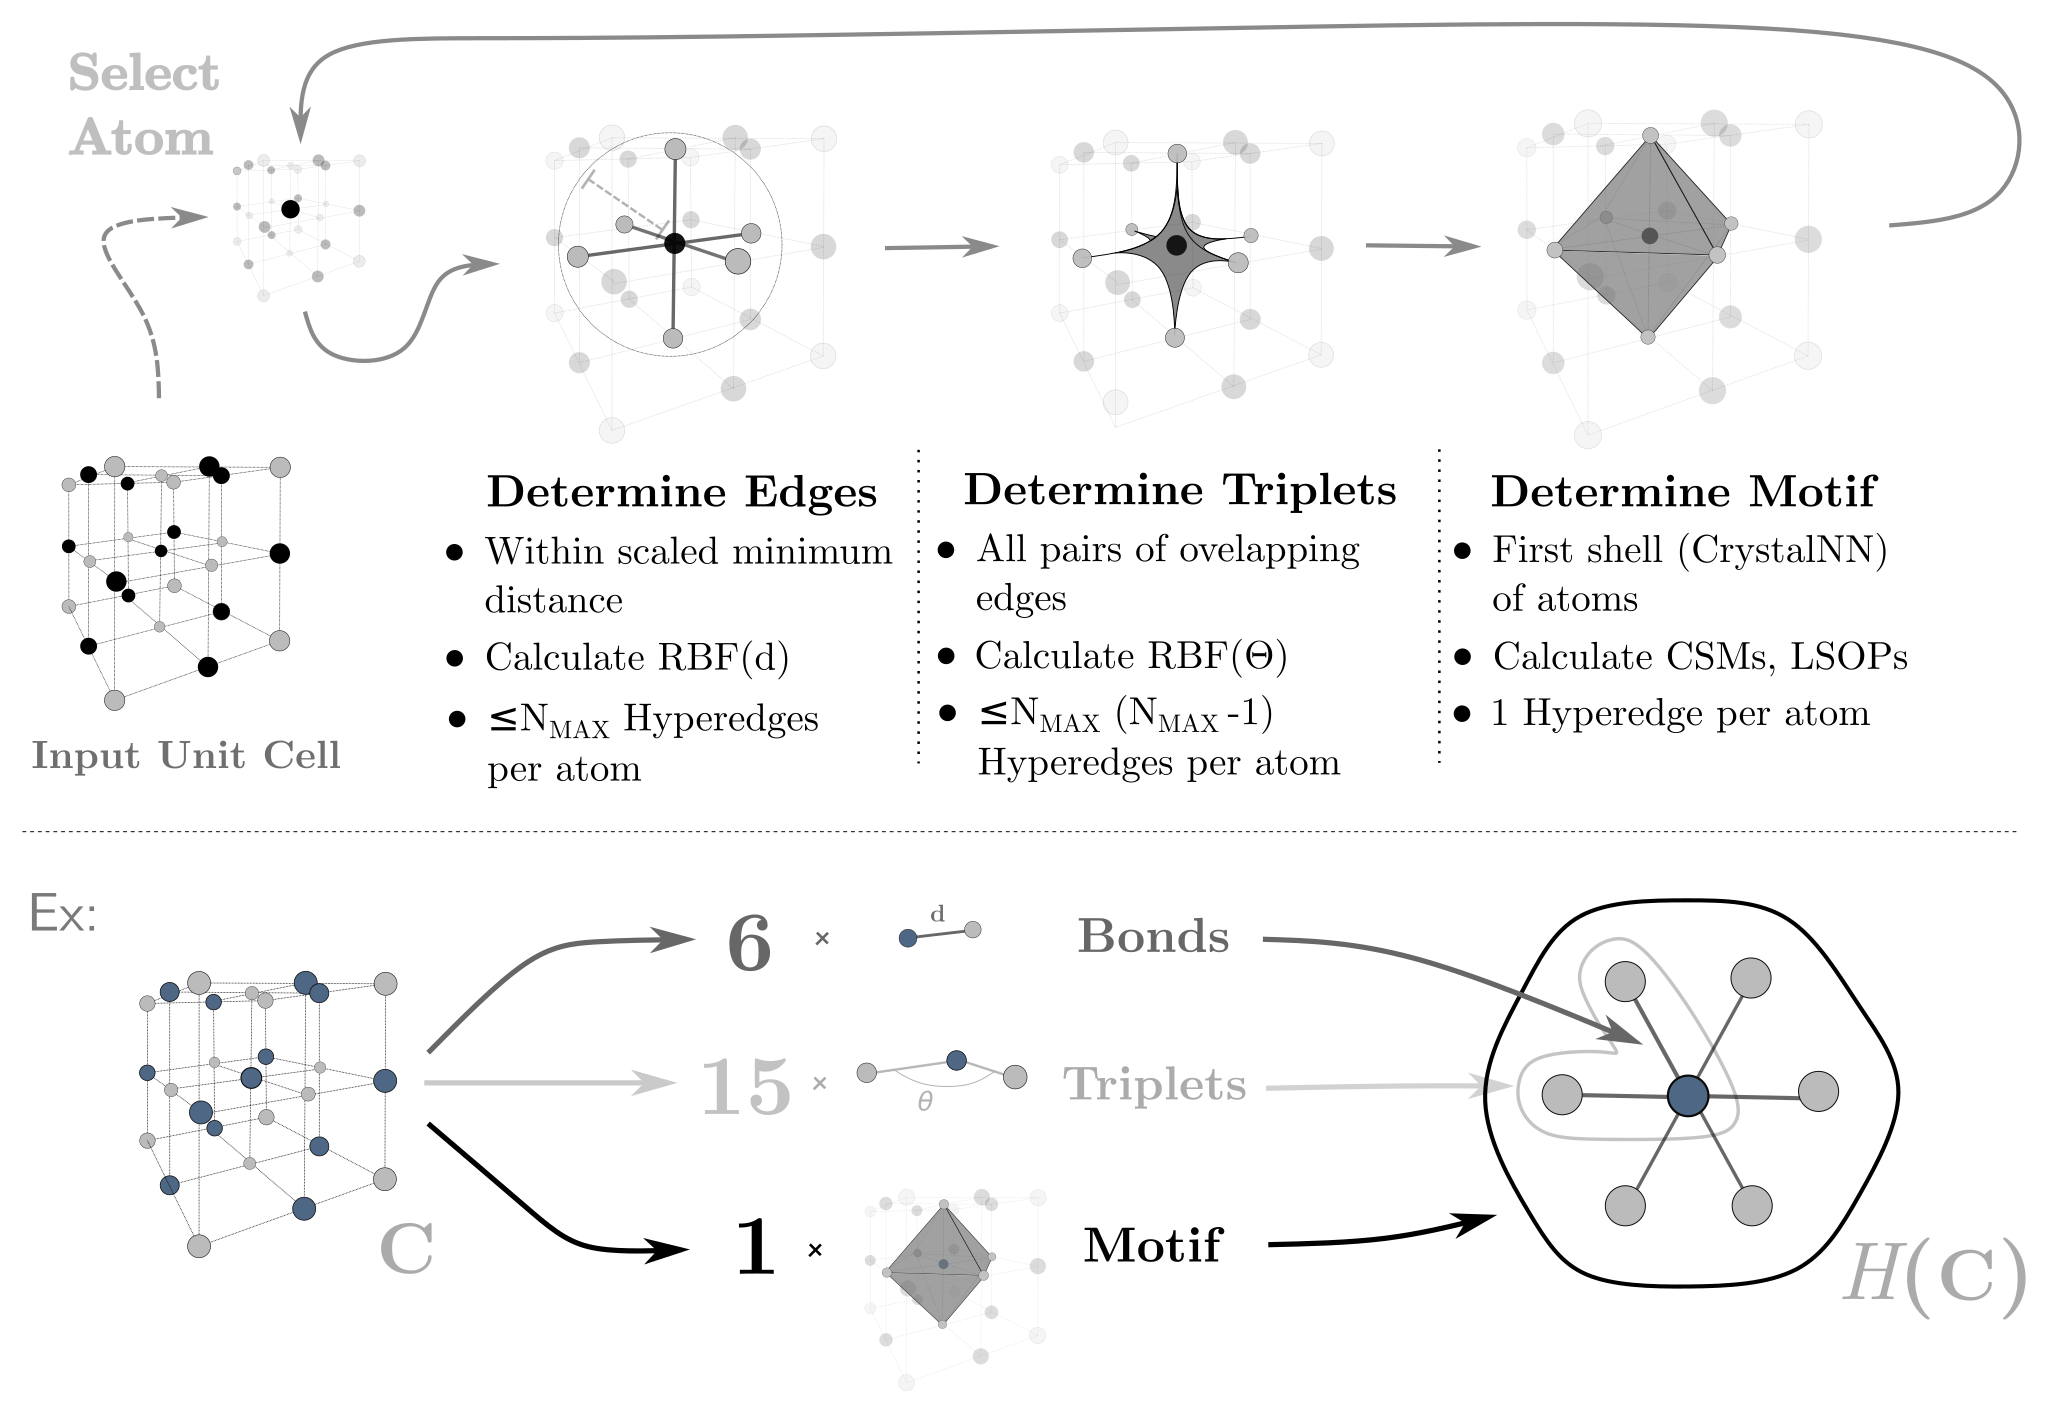
\includegraphics[scale=0.27]{crystal_hgraph_ex+revamp3.pdf}
	\caption{Typical construction loop for a crystal hypergraph. First, pair-wise bonds/edges are determined, then triplets are derived from overlapping pairs of bonds, and finally motifs are determined as first-shells of neighbors by some (generally more restrictive) criteria. Features for each and upper bounds on numbers of hyperedges for each type are also listed. Note that RBF abbreviates radial basis function (such as Gaussian, Bessel, etc.); CSM, continuous symmetry measure; and, LSOP, local structure order parameter.}
	\label{fig:hypergraph-loop}
\end{figure*}

\subsubsection{Bond Edges}
Bonds, or pair-wise atomic connections, are determined in the same manner as in a crystal graph. In the results below, we choose edges from a maximum number of neighbors $N_{max}=12$ found within a shell of radius $r_{max}=6\AA$. 
%The feature associated with such edges is a Gaussian expansion of the distance, with a range from 0 to 6 Angstrom and a dimensionality of 40.

\subsubsection{Triplet Hyperedges}
Triplet hyperedges are then formed from the set of bonds. For each set of bonds connected by one node, a triplet hyperedge is formed. The feature of these triplet hyperedges is also a Gaussian expansion, though now of the angle formed by the unit vectors of the two bonds \cite{alignn}.
Triplet hyperedges give us a way to incorporate some angular resolution into our representation scheme in a coordinate-system-invariant manner.
For a node with $N$ bonds then, there will be $N(N-1)/2$ triplets. Thus, the price we pay for complete angular resolution of any two bonds is a quadratic increase in the number of hyperedges. For a comparison between our inclusion of triplet information and the more usual construction by way of a line-graph, see Supplementary Note S4.


%\begin{center}
%\includegraphics[scale=0.15]{revamp.pdf}

%OR


%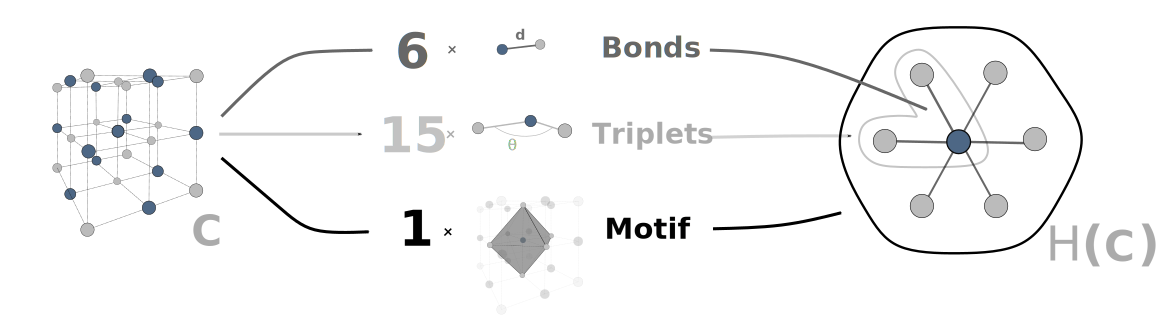
\includegraphics[scale=0.13]{revamp2.pdf}

%\end{center}


\subsubsection{Motif Hyperedges}
Motif determination may be achieved by a wide range of functions, and is akin to an algorithmic determination of coordination number \cite{coordination_comp}. Here, we use a modified Voronoi algorithm with a cut-off radius implemented as CrystalNN in pymatgen.
Note this is a much stricter algorithm than that used to determine edges and triplets, since the motifs features depend heavily on the selected first-shell.

The features of these motifs are a concatenation of Zimmerman's 34 local structure order parameters \cite{orderparam1,orderparam2}, and continuous symmetry measures \cite{csm_polyhedra} (e.g. 'distance to a perfect shape') for 59 common coordination environments (see Supplementary Note S1). In essence, both are just sets of quantitative measures designed to describe 3 dimensional physical shape. 
Motifs give us a way to describe the local geometry of sites in material systems with much fewer hyperedges. Since each node will contribute one motif hyperedge, for a crystal with $N_{\text{nodes}}$ nodes, we just have $N_{\text{nodes}}$ motifs. 


\section{Crystal Hypergraph Convolution}

We now must consider a message passing framework analogous to \textit{Gilmore, et al} \cite{mpnn} but applying to hypergraph structures. That is, we now have:
\begin{align*}
	m_v^{t+1}&=\sum_{h_j\in \mathcal{N}(v)} M_t(n_v^{t},h_j^{t},\lbrace n_w^t \vert n_w \in h_j \rbrace),\\
	n_v^{t+1}&=U_t(n_v^t,m_v^{t+1}),\\
	\hat{y}&=R(\lbrace n_v^T\rbrace),
\end{align*}
so that each node is still updated according to some layer-wise update function $U_t$, aggregating messages $m^{t+1}$ formed from origin node features, hyperedge features $h_j$, and hyperedge neighborhood features $n_w \in h_j$. This update occurs node-wise and then after $T$ layers, some readout function $R$ is used to output the corresponding predicted value $\hat{y}$, which utilizes the set of learned node features.


%where $m_v^{t+1}$ is the message formed for node $v$ in the $(t+1)$-th layer; $M_t$ is the message function; $n_v^t$ is the node representation; $h_j^t$ is the representation of the $j-$th hyperedge feature with a neighborhood contain node $n_v$, which compose the 'neighborhood' of node $v$, $\mathcal{N}(v)$; $U_t$ is the representation update function; and $R$ then is the readout function giving the predicted value $\hat{y}$.

The biggest difference here is that we now need a message forming function $M_t$ that accounts for a set of node features $\lbrace n_w^t \vert n_w \in h_j \rbrace$ which may vary in size between different hyperedges (even of the same type). This stands in opposition to the case of regular edges, where we are assured a fixed size of two nodes per edge. 

One approach would be to fix the dimensionality of each type of hyperedge, or have a different convolutional operator for each different size hyperedge (as is effectively the approach taken with line graph networks \cite{linegraph_general}). Here, however, we wish to maintain generality in edge size so we need not fix hyperedge sizes for hyperedge type, since structures of different sizes may be described by similar metrics. For example, we may wish that motifs resembling polyhedra with different numbers of vertices are described by common sets of features.

%Note that we may also wish to update hyperedge representations of one type according to other hyperedges of the same or other types. As an example, we may desire the two bonds forming a triplet to be updated from messages based on the angle they form. Or, we may hope to update a motif's representation based upon the unit cell it resides in. 

%These connections between the same or different orders of hyperedge may be defined based upon inclusion and/or contact. In the case of the bond-triplet-bond interaction, we may determine the relationship between these hyperedges by forming messages for bonds included in triplets. Furthermore, we may care to relate triplets that are touching each other, or mutually contain one or more nodes.

Of course, there should be different message and update functions for each different order structure (bonds, triplets, motifs, etc.) with different features. This is accounted for by treating the data as a heterogeneous graph, with different hyperedge types. Below, we consider three strategies that allow us to apply our convolutional operator to hyperedges of arbitrary size.


\subsection{Three Possible Approaches to Hyperedge Convolution}

Three general approaches for message passing that account for this multi-order nature have been considered in this work: \textbf{1.} the construction of a hyperedge relatives graph, upon which regular graph convolution may be applied; \textbf{2.} total exchange hyperedge message convolution, which completely generalizes the CGCNN \cite{cgcnn} and ALIGNN \cite{alignn} models to hypergraphs; and \textbf{3.} neighborhood aggregation, which balances performance of the former approach by forming a single neighborhood feature for each hyperedge.

Each approach has a different computational cost in terms of the total number of messages, along with a potentially different practical definition of a hypergraph. These considerations are presented below, with a specific convolutional structure and empirical results on common test datasets presented after.

%Note also that through testing, a guiding principle was learned for hyperedge messages: each order of hyperedges should contribute the same number of messages to each node. That is, each node should be updated by some global, fixed number of messages for that order of hyperedges.

\subsubsection{Hyperedge Relatives Graph}
We may define a dual graph $\mathcal{D}(h)$ to a hypergraph $h$ to be a graph in which nodes represent the hyperedges of the hypergraph, and connections represent the overlap of respective hyperedge neighborhoods. 
In the case of a crystal hypergraph with heterogeneous hyperedges, this dual graph is a graph with heterogeneous nodes. We term this heterogeneous dual graph of a crystal hypergraph the relatives graph for simplicity. Atomic features may be included in this framework by adding a singleton hyperedge for each node.

The definition of the relatives graph allows us to perform the usual methods of graph convolution on hyperedge features. Such an approach also allows us to define our relatives graph as we would a graph, with just a standard edge index.

\begin{figure*}
	\centering
	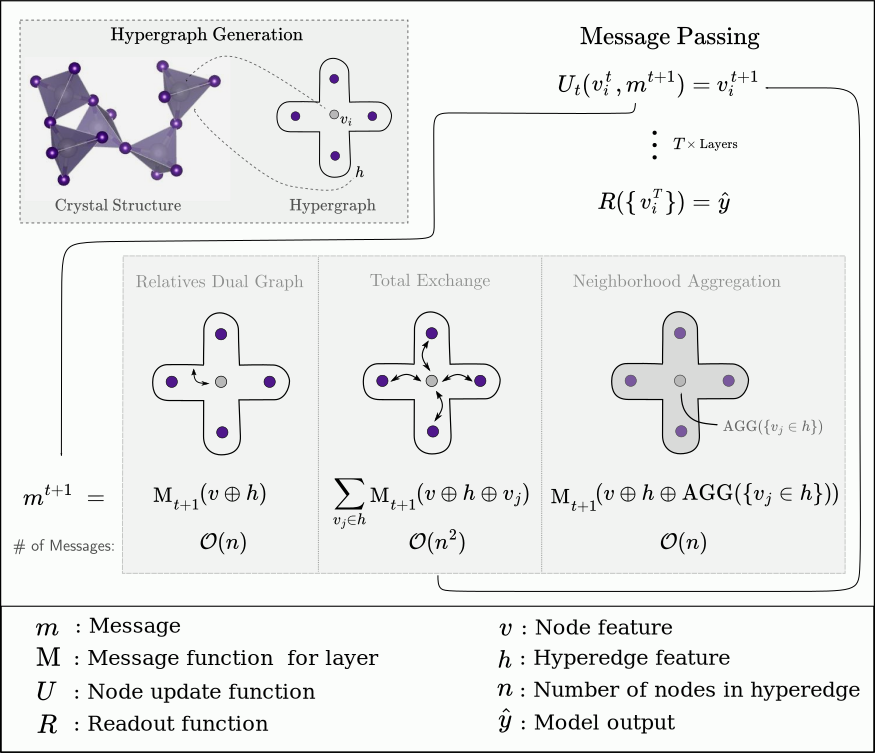
\includegraphics[scale=.68]{HMPNN_loop.pdf}
	\caption{Overview of three possible message functions $M$ for nodes that generalize the message function in \cite{mpnn} to hyperedges $h$ with more (or less) than two nodes. %Here, $n$ represents the average number of nodes in a hyperedge and the scaling relation is for the total number of messages exchanged for each hyperedge, per layer. 
	$\text{AGG}$ specifies some aggregation function acting on the set of node features in the hyperedge, such as max, min, or average.}
	\label{fig:hmpnn}
\end{figure*}

However, this approach lacks the interaction of neighboring features in convolution via the connecting hyperedge. That is, without a clear definition of the edge attribute, messages are generally of the form below:
$$
m_v^{t} = \sum_{h_j\in \mathcal{N}(v)}M_t(n_v^{t},h_j^{t})
$$
in which we simply discard the neighborhood of other node features contained in the hyperedge.

Computationally, this approach has a total number of messages that scales linearly with average hyperedge size, since each hyperedge only contributes one message to each node it contains.
Accounting only for node-hyperedge connections in a relatives graph derived from a hypergraph with $m$ hyperedges of average order $n$, the total number of messages per convolution will scale as $\mathcal{O}(nm)$.

\subsubsection{Total Exchange Message Passing}
Of course, we may wish to incorporate the neighboring features of some representation via their connecting hyperedge. This may be accomplished by simply forming a message for every pair of connected representations along with their connecting hyperedge's representation.
$$
m_v^{t} = \sum_{h_j\in \mathcal{N}(v)} \sum_{n_w \in h_j } M_t(n_v^{t},h_j^{t}, n_w^t),
$$
%Note that this method completely generalizes previous approaches based on line graph convolution, or nested graph networks
Here, though, we have introduced a new summation which may drastically increase the number of messages for larger hyperedges. In this scheme, if each hyperedge contains an average of $n$ nodes and there are $m$ hyperedges, the total number of messages exchanged per node-wise convolution will scale as $\mathcal{O}(n^2m)$.

%This approach also requires a different practical definition of the hypergraph.  Instead of a two dimensional index set, we now define a three dimensional index set, relating the origin node, the connecting hyperedge, and the connected node.

\subsubsection{Neighborhood Aggregation}
Since the number of messages will scale tremendously with larger hyperedges in the framework described above, we may seek a way to incorporate the neighborhood of contained node features of a hyperedge into a single message. In this case, we may form a single `neighborhood feature' representative of all contained nodes of a hyperedge by way of an aggregation function. This aggregation function takes as input a variable number of node features and returns a single feature of fixed dimension. Here then, we use message functions of the form: 
$$
m_v^{t+1}=\sum_{h_j\in \mathcal{N}(v)} M_t(n_v^{t},h_j^{t},\text{AGG}\big(\lbrace n_w^t \vert n_w \in h_j \rbrace\big)
$$
where $\text{AGG}$ denotes some order-invariant function on a set of node features, such as component-wise minimum, maximum, average, or a combination of these with learnable weights. The use of an aggregation function here thus allows for the passing of one message per hyperedge, while accounting for the entire environment of local node features in the hyperedge.
This results in a set of node-wise messages that scales linearly with the average size of hyperedges, so that we now have a relationship of order $\mathcal{O}(nm)$ again.

\subsection{Model Architecture}
In our CHGCNN model, initial atomic features were those used in CGCNN \cite{cgcnn}, consisting of a concatenated set of one-hot encoded atomic properties. For bond features, we used a Gaussian expansion of interatomic distance of dimension 40 ranging from 0 to 6 \AA, triplet features were a Gaussian expansion of the cosine of bond angle, also of dimension 40, and motif features were a concatenation of 93 scalar order parameters and continuous symmetry measures. In the model considered in this work, initial node and hyperedge features were first passed into a linear embedding layer (with no activation function) with an output dimension of 64. 

These embedded features were then fed into a set of Crystal HyperGraph Convolutional (CHGConv) layers which utilize the neighborhood aggregation method presented above (see Supplementary Note S2). In CHGConv, we use a set of CGConv \cite{cgcnn} layers applied to consecutively larger hyperedge types, taking as input the origin node of the hyperedge, the connecting hyperedge feature as the edge feature, and an aggregated set of neighborhood features as the connected node feature. Inspired by \cite{chemgnn}, the $\text{AGG}$ function chosen for neighborhood aggregation through message passing on hyperedges was a combined set of component-wise maximum, minimum, average, and standard deviation, all with learnable attention weights. In this manner, for every CHGConv layer, the atoms are updated by each hyperedge type chosen once (see Fig. \ref{fig:architecture}). Note that each CGConv for different hyperedge types have independent trainable parameters. 

These learned node features are then mean pooled to form a crystal vector, which is passed to a fully connected layer and then projected down to a one-dimensional (scalar) output for regression. In the case of classification tasks, the fully connected layer, after mean pooling, utilized a dropout mechanism and output a probability distribution of classes by way of a softmax activation function.

\begin{figure*}
	\centering
	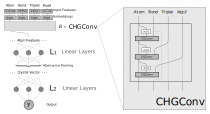
\includegraphics[scale=.75]{arch_horiz.pdf}
	\caption{Example architecture for the crystal hypergraph convolutional network implemented in this work. Essentially, the model is a generalization of CGCNN's \cite{cgcnn} model architecture with CGConv being replaced by $R$ hypergraph convolutional layers (CHGConv). Here, CHGConv updates nodes first according to edges (bonds), and then according to triplets or motifs. }
	\label{fig:architecture}
\end{figure*}


\section{Results \& Discussion}
Crystal hypergraph networks provide a unique opportunity to investigate the importance of different order structures in the prediction of various material properties. Specifically, we may compare performance between models based on different types of hyperedges to probe the relevance of certain structures (e.g. motifs vs. triplets) in material property prediction. From the different hyperedge types considered here, we build three different models based on the architecture given in Fig. \ref{fig:architecture}.
We first test a basic bond-only network equivalent to CGCNN, and compare its performance against two models incorporating two types of hyperedges: bond-and-triplet and bond-and-motif models. 
%We consider three models incorporating only one type of hyperedge: bond-only, triplet-only, and motif-only; as well as two models incorporating two types of hyperedges: bond-and-triplet, and bond-and-motif models. 
For compound models (including more than one hyperedge type) each CHGConv layer performs convolution over the hyperedges in ascending order of hyperedge size. These models were each trained on sets of training data from  MatBench (v0.1) \cite{matbench}. Details on the hyperparameters and training protocol can be found in the Supplementary Note S3. Note that models using both motif and triplet-level edges, in general, diverged through training or did not perform any better than models using just motifs or triplets. As such, we only compare models using one or the other here. For all tests, datasets were split into 80\% train / 20\% test subsets across 5 folds. The training subsets were then further split into 90\% train / 10\% validation sets, where the model with the best performance on the validation set (withheld through training) was then used to predict the values of the final test sets. Note that MatBench provides fixed fold splits for benchmarking purposes. Performance on each fold is reported in Supplementary Section S9.

We first focus on the comparative performance of models incorporating only bonds, models incorporating both bond-and-motif hyperedges and models with both bond-and-triplet hyperedges on five smaller MatBench (v0.1) target datasets \cite{matbench}. Mean absolute error (MAE) on test sets for these tasks are reported in Table \ref{fig:matbench_table}. These five datasets consist of the following targets: the highest frequency phonon peak $\omega_p$ for 1,265 materials, refractive indices $n$ for 4,764 materials, formation energies $E_f$ for a set of 18,829 perovskite materials, and 10,987 bulk and shear moduli, $K_{vrh}$ and $G_{vrh}$, respectively.
On all tasks of these smaller sets, the larger models incorporating both bonds and higher-order hyperedges performed best, with the motif-based models performing best overall. 
For refractive index prediction, the motif-based models had an average MAE of 0.432 across the test sets compared to an MAE of 0.440 for the bond-and-triplet model, with both showing improvement over the bond-only model with an MAE of 0.448. Perovskite formation energy prediction results were very close for the three models, while the bond-and-motif model again had the best performance with an MAE of 0.0424 eV/atom, the bond-and-triplet model was close behind at an MAE of 0.0427 eV/atom, both showing only a slight improvement over the bond-only model's performance with an MAE of 0.0433 eV/atom. However, since perovskites are a class of materials with a relatively standard structure, it should be unsurprising that the inclusion of additional structural information has little to no effect on performance.
In the prediction of highest frequency phonon peak, the bond-and-motif model had the best performance with an average MAE of 52.9 cm$^{-1}$ across test sets compared to 60.7 cm$^{-1}$ for the triplet based model and 57.0 cm$^{-1}$ for the bond-only model. For elastic targets, motif based models boasted average MAEs of 0.0805 Log$_{10}$(GPa) and 0.0635 Log$_{10}$(GPa) on the test sets of bulk moduli $G_{vrh}$ and shear moduli $K_{vrh}$, respectively. This is compared to the performance of the bond-and-triplet models with MAEs of 0.0846 Log$_{10}$(GPa) and 0.0666 Log$_{10}$(GPa) on $G_{vrh}$ and $K_{vrh}$, with only the latter being an improvement over the bond-only models with MAEs of 0.0839 Log$_{10}$(GPa) and 0.0681 Log$_{10}$(GPa). This may be indicative of the importance of such information in the relation of stress to infinitesimal strain, since the local environments of atoms would be of particular importance in considerations of bulk response (that is, calculations of $K_{vrh}$) though, perhaps, less so in considerations of shear response ($G_{vrh}$).

%%%MAIN TEXT%%%%
%\subsection{Tables}
%Tables typeset in RSC house style do not include vertical lines. Table footnote symbols are lower-case italic letters and are typeset at the bottom of the table. Table captions do not end in a full point.\cite{Arduengo1992,Eisenstein2005}


%\begin{table}[h]
%	\small
%	\caption{\ An example of a caption to accompany a table}
%	\label{tbl:example1}
%	\begin{tabular*}{0.48\textwidth}{@{\extracolsep{\fill}}lll}
	%		\hline
	%		Header one (units) & Header two & Header three \\
	%		\hline
	%		1 & 2 & 3 \\
	%		4 & 5 & 6 \\
	%		7 & 8 & 9 \\
	%		10 & 11 & 12 \\
	%		\hline
	%	\end{tabular*}
%\end{table}

%Adding notes to tables can be complicated.  Perhaps the easiest method is to generate these manually.%\footnote[4]{Footnotes should appear here. These might include comments relevant to but not central to the matter under discussion, limited experimental and spectral data, and crystallographic data.}

%\begin{table*}
%	\small
%	\caption{\ An example of a caption to accompany a table \textendash\ table captions do not end in a full point}
%	\label{tbl:example2}
%	\begin{tabular*}{\textwidth}{@{\extracolsep{\fill}}lllllll}
	%		\hline
	%		Header one & Header two & Header three & Header four & Header five & Header six  & Header seven\\
	%		\hline
	%		1 & 2 & 3 & 4 & 5 & 6  & 7\\
	%		8 & 9 & 10 & 11 & 12 & 13 & 14 \\
	%		15 & 16 & 17 & 18 & 19 & 20 & 21\\
	%		\hline
	%	\end{tabular*}
%\end{table*}


\begin{table*}\small
	\begin{tabular*}{\textwidth}{@{\extracolsep{\fill}}cccccc}
		\hline 
		$\quad$ & $\omega_p$  & $n$  & $E_f$  & Log$_{10}$($G_{vrh}$) & Log$_{10}$($K_{vrh}$) \\
		Hyperedge & (\textit{1,265}) &  (\textit{4,764}) & (\textit{18,829}) & (\textit{10,987}) & (\textit{10,987}) \\
		Types & MAE (cm$^{-1}$) & MAE & MAE (eV/Atom)& MAE (Log$_{10}$GPa)& MAE (Log$_{10}$GPa)  \\
		\hline
		Bond-only & 57.0& 0.448 & 0.0433 & 0.0839 & 0.0681\\
		Bond \& Triplet & 60.7& 0.440 & 0.0427 & 0.0846 & 0.0666 \\
		Bond \& Motif & \textbf{52.9}& \textbf{0.432} &\textbf{0.0424} & \textbf{0.0805} & \textbf{0.0635}\\
		\hline
		Bond Messages & 112,596 & 960,912 & 1,135,680 & 1,061,628 & 1,061,628\\
		Triplet Messages & 927,135 &5,756,865& 13,032,891 & 10,281,801  & 10,281,801\\
		Motif Messages & 9,383 & 80,076 & 94,640 & 88,469 & 88,469 \\
		\hline
	\end{tabular*}
	\caption{Test results averaged over 5 folds of nested cross-validation for five MatBench target sets: highest frequency phonon peak $\omega_p$, refractive index $n$, perovskite formation energy $E_f$, and bulk moduli $K_{vrh}$ and shear moduli $G_{vrh}$. Note that the italicized numbers below the target name in parentheses correspond to the total size of each dataset, while test results are reported as an average on the test sets of the 5 MatBench \cite{matbench} folds. Best results are indicated in bold. The number of messages contributed per layer for each type of hyperedge is listed below the line dividing the tables elements for each target set, respectively.}\label{fig:matbench_table}
\end{table*}

 %This is corroborated by the difference in performance between motif and triplet models on both tasks, since motif information seems comparable in prediction of bulk moduli with an MAE of 0.073 Log$_{10}$(GPa) for the motif model (compared to 0.071 Log$_{10}$GPa for the triplet-based model), but less so in the prediction of shear moduli with an MAE of 0.095 Log$_{10}$(GPa) (compared to 0.088 Log$_{10}$GPa). 


To see if the improved perfromance of motif-based models generalizes to larger data sets, we now compare the performance of bond and bond-and-motif models on three more target properties for a much larger sets of
materials from the Materials Project database \cite{matproj}, again provided by MatBench (v0.1), with targets including formation energy $E_f$, band gap $E_g$, and metallicity.  Results for this set of tests are reported in Table \ref{fig:mp_table} with MAE reported for regression tasks and area under curve (AUC) for classification tasks. 
For the Materials Project datasets, the bond-and-motif model performed best on the band gap and metallicity target sets, with the bond-only model then performing best on the formation energy task. In the prediction of band gap, the bond-and-motif model performed better than that without motifs, with an MAE of 0.0231 eV vs. an MAE of 0.0259 eV for the bond-only model. This trend also held for the metal/nonmetal classification task, with the best performance on the test set again by the bond-and-motif model with an AUC of 0.958, compared to an AUC of 0.954 for the bond-only model. In the prediction of formation energy, the bond-and-motif model and bond-only model had prediction MAEs of 0.0397 eV/atom and 0.0377 eV/atom, respectively.  



\begin{table*}
	\begin{tabular*}{\textwidth}{@{\extracolsep{\fill}}cccc}
		\hline
		 & $E_f$ & $E_g$ & Metal/Non-metal Classification \\
		Hyperedge & \textit{(132,752)} & \textit{(106,113)}  & \textit{(106,113)}\\
		Types & MAE (eV/Atom) & MAE (eV) & AUC \\
		\hline
		Bond-only & \textbf{0.0377} & 0.259 & 95.4\% \\
		%Bond \& Triplet &  \textbf{0.0484} & \textbf{0.325 } & \textbf{93.3\%}\\
		Bond \& Motif &  0.0397 &\textbf{ 0.231} & \textbf{95.8}\%\\
		\hline
		Bond Messages & 46,435,896& 38,219,808 & 38,219,808 \\
		Motif Messages &3,869,658 & 3,184,984 & 3,184,984 \\
	\end{tabular*}
	\caption{Test results for three Materials Project target sets: formation energy $E_f$, band gap $E_g$, and metallicity. Note that the italicized numbers below the target name in parentheses correspond to the total size of each dataset, while test results are reported as an average on the test sets of the 5 MatBench \cite{matbench} folds. Best results are indicated in bold. The number of messages contributed per layer for each type of hyperedge is listed below the line dividing the tables elements for each target set, respectively.}\label{fig:mp_table}
\end{table*}



%\section{Conclusion}
%Graphs are a relatively restrictive representation system for crystal structures, which have clear structures beyond just pair-wise interaction. Especially in the manner they are most usually constructed, crystal graphs are often of low geometrical resolution; in that related but distinct structures may map to the same crystal graph.

%Other modern works often address this lack of geometrical resolution by auxiliary, iteratively derived, line graphs, in which angles of triplets, dihedrals, etc. may be associated as features. One problem with such approaches, however, is the quadratic increase in graph size with each iterative construction.

%The primary argument of this paper then is that hypergraphs are a more natural representation of crystal structures that allow us to incorporate this lost geometrical information for different substructures of our choice.  Hypergraphs allow us to explicitly incorporate coordinate invariant features with higher order structures, such as triplets and motifs, as feature vectors associated with a heterogeneous hyperedge set.

%The introduction of a new representation scheme requires a generalization of previous convolutional methods, most generally described by the MPNN framework. Here, we considered three approaches to generalize the message passing framework to variable order hyperedges. These allow us to perform supervised learning tasks on crystal hypergraphs.

%A basic crystal hypergraph convolutional neural network (CHGCNN) was implemented and tested with and without bond and motif hyperedges. These results were compared for several different material property target sets of various sizes.

%Structural tasks seemed to benefit greatly from the inclusion of explicit geometrical information in the way of motif-level features. However, electronic tasks seemed to benefit much less from motif-level information, sometimes performing better with only bond-type edges. These tendencies seemed to be particularly prevalent in smaller datasets though, suggesting datasize scaling effects may also be contribute to this trend.

Perhaps the strongest point to be made in regard to these results is that for most tasks, motif information contributed to comparable or better performance than triplet-level results. This is at a significantly lower computational cost, in terms of the total number of messages exchanged through convolution, since the number of motifs is simply the number of atoms $n$, whereas the number of triplets scales with the average number of bonds per atom $N$ as $N(N-1)/2$.

A similar observation was made in the AMDNet architecture \cite{amdnet}, where motif information (included via an additional 'motif graph' for each material) also improved performance on most tasks, but here we compare results directly to the inclusion of bond angles via triplets.
Our results indicate that one local neighborhood feature per atom may be sufficient to describe the local geometries of atoms for many predictive tasks, as opposed to the more data-intensive triplet representation scheme usually employed (often by way of line graphs). Taking this as a learned guiding principle, future crystal representations may benefit from reduced size while being assured similar geometric resolution. However, it should be noted that the greatest improvements seen here were on smaller datasets, suggesting the inductive bias of the motif-level hyperedges yields diminishing returns with larger datasets. This suggests that with large enough training data sets, continuous convolution filters for hyperedges encoding distance or angle alone may sufficient for larger targets. However, given the intrinsic difficulty of the production of most target data in the materials science, the specific methods presented here may still prove beneficial in many applications. 



\section{Conclusions}
State-of-the-art GNN models applied to material property prediction often represent material systems as graphs with relatively low geometrical resolution. This low resolution is often increased by associating bond angles with auxiliary line graphs derived from the graph itself. The primary argument of our work is that hypergraphs are a more natural representation of material structures that allow us to explicitly incorporate geometrical information with different substructures of choice in one unified representation. The results suggest that such an approach allows for a substantial decrease in computational cost compared to line-graph or triplet methods, by incorporating such geometrical information with single local environment hyperedges for each node as opposed to triplets of atoms for each pair of overlapping bonds. This is shown within one unified framework to have comparable performance on a number of common predictive tasks.
In principle, these motif-level hyperedges may be added to any existing atomistic graph neural network. The results in this work further suggest that these additional hyperedges may improve performance for these models across many supervised predictive tasks, with a relatively small computational cost since the motif-level hyperedges contribute substantially less messages per convolutional layer compared to the number of bonds.

Future works may investigate more powerful hypergraph convolutional operators that automatically detect motifs \cite{contrastivelearn_motif, motifexplore, motife3nn}; or apply this framework to molecular systems \cite{ molecule2, molecule3} with functional groups. Inter-order convolution may also be of interest for certain tasks, where different hyperedge types may update each other's representations as opposed to just atom representations. Note that inter-order convolution would allow for a complete generalization of previous line-graph convolution schemes, where triplets effectively update their respective bonds' representations through convolution, as in \cite{alignn, congn}. Other order structures (beyond motif-level) may also be of interest, such as hyperedges representing defect complexes or entire unit cells. Equivariant features and convolution \cite{e3nn, tfn, o3transformer1} may also be incorporated for the prediction of coordinate-system dependent properties of materials from hypergraph representations, with the present work being focused on coordinate-system invariant features and targets. 


\section{Data Availability}
The code used in this paper's results were built on pytorch-geometric and can be found in the following Github repository:
%\hyperlink{https://github.com/qmatyanlab/CHGCNN}{https://github.com/qmatyanlab/CHGCNN}
https://github.com/qmatyanlab/CHGCNN. The processed data including bond, triplet, and motif features is available in a Zenodo repository with DOI: 10.5281/zenodo.14756640.


\section{Acknowledgments}
This work is supported by the U.S. Department of Energy, Office of Science, Basic Energy Sciences, under Award No. DE-SC0023664. This research used resources of the National Energy Research Scientific Computing Center (NERSC), a U.S. Department of Energy Office of Science User Facility located at Lawrence Berkeley National Laboratory, operated under Contract No. DE-AC02-05CH11231 using NERSC award BES-ERCAP0029544.


%\bibliography{chgcnn}
\printbibliography

\medskip


\newpage

\appendix

%\section{Motif Determination}
%Motifs are determined according to criteria similar to that used in bond determination. Namely, interatomic distance, Voronoii tesselations, and solid-angles of Voronoii faces are still relevant. Despite this similarity in potential criteria, testing showed more restrictive approaches to motif determination resulted in better performance on validation sets. This stands in contrast to edge determination, where the continuous order convolution operators may be used to 'pick' the more important bonds from a large, loosely defined set of bonds, by the corresponding distance feature.

%Several different schemes were tested for a single task (band gap) with a relatively large amount of samples (150,000) and compared. First, the same criteria as bonds was applied (that is, all within a certain radius, up to a maximum number of neighbors), which performed worst. Second, a scaled minimum radius cutoff was applied, where for each site, the motif was determined to be all those neighbors within a factor of $\alpha=1.2$ times the closest neighbor's interatomic distance (for that site) $r_{\text{min}}$. Finally, the more restrictive criteria of CrystalNN, as defined in \cite{crystalnn}, was applied, which applies a scaled distance cutoff as well as a scaled solid angle cutoff. Results are displayed below for comparison. Note that all models used both bond and motif-level information (where bond criteria was held constant through all)

%\begin{center}

%\begin{tabular}{c|ccc}

%Motif Criteria & Naive & Scaled $r_{\text{min}}$& CrystalNN \\
%\hline
%Best MAE (eV)  \\
%\end{tabular}
%\end{center}
%The more restrictive definitions of motifs increased in performance incrementally. This is likely since the larger motifs would tend to 'smoosh' the atomic information too much through aggregation of neighborhood features and messages.



\end{document}
